



\section{Wireless networks}

In this section, communication networks are presented, with special attention to wireless technologies. 
An historic overview is presented in \ref{subs:331} to illustrate the relevant milestones to achieve nowadays communication networks.  
In \ref{subs:332} and \ref{subs:333} are presented the current solutions for wireless communication.
The evaluation of wireless networks is presented in \ref{subs:334} and \ref{subs:335}, first with the presentation of the \ac{KPI} and then with the identification of the simulators and emulators.


\subsection{Network technologies – historic overview}
\label{subs:331}
The beginning of modern communication systems is marked with the expansion of the telegraph, having an important milestone happening in 1858 with the first communication between USA and UK. Since then, the telephone has emerged and widely used; the wireless communication was successfully established in 1901 and, decades later, worldwide communication had the support of satellite communication systems.

One important area of communications is the computer networks, and in particular, the internet where it is used in several aspect of business (such as advertising, production, shipping, planning, billing, and accounting, \cite{comer2008}). In 1980 the Internet was a research project involving few dozen sites and currently the Internet is an important part of people’s communication.

Currently, a computer network is well organized, having a well-structured \ac{IP} that defines how data passes through layers, as represented in figure \ref{fig:comer2008}.

	\begin{figure}[h!]
	\centering
	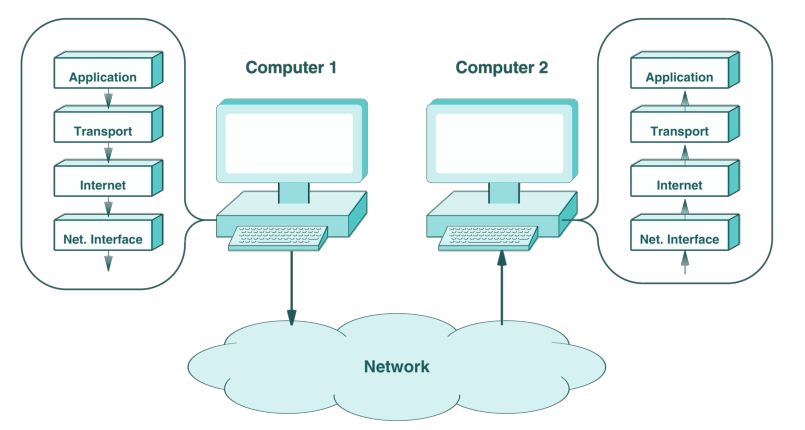
\includegraphics[width=0.8\textwidth,keepaspectratio]{figures/33.WirelessN/comer2008}
	\caption{Representation of data flow in a computer network. Adapted from \cite{comer2008}.}
	\label{fig:comer2008}
\end{figure}


\subsection{Current Wireless technologies and standards}
\label{subs:332}
The following sections will cover the wireless communications in smart metering systems, starting with the low-rate and low-power communications applied on smart meters and ending with the high-rate communications (and consequently higher costs and power than low rate communications). With the increasing on demand for higher bandwidth, broadband technologies such as mobile WiMAX, IEEE 802.16e and broadband \ac{PLC} are expected to be considered and used in newer installations, \cite{Mohassel2014}.


%As the demand for bandwidth increases, broadband technologies such as IEEE 802.16e, mobile WiMAX and broadband PLC are going to play a key role in newer installations, \cite{Mohassel2014}.

\subsubsection{IEEE 802.11 (\ac{WLAN} or Wi-Fi)}

IEEE 802.11 is the standard for the information exchange between systems and for the telecommunications. The coverage area of this technology is on local and metropolitan area networks (LANs and MANs). The specific requirements are on the Medium Access Control and on Physical Layer. The most popular versions of this standard is the IEEE 802.11b and IEEE 802.11g, that differs in the modulation technique (\ac{DSSS} technique versus  \ac{OFDM} modulation technique). The data rates are, respectively, 11 Mbps and 54 Mbps, \cite{Usman2013, ieee2012}.



\subsubsection{IEEE 802.15.4 (ZigBee)}

The standard IEEE 802.15.4 imposes conditions in the physical layer and media access control focusing on low-rate (up to 300 kHz) wireless personal area networks. Developed by the Zigbee Alliance and covering the specifications of the IEEE 802.15.4 on the physical layer and the medium access control, Zigbee is a commonly used for low power wireless communication technology. It operates on the \ac{ISM} bands of 868 MHz, 915 MHz and 2.4 GHz adopting \ac{DSSS}, \cite{Usman2013}.



\subsubsection{DASH7}

On the low-rate field of research, an alternative to Zigbee is the DASH7. Using the ISO/IEC 18000-7 standard to support this wireless sensor network technology, DASH7 is developed to reach active Radio Frequency Identification Devices (RFIDs) and operates at 433MHz band. The advantage is the typical range of 250m (could achieve 5 km) and has a typical and maximum data rates of 28 kbps and 200 kbps, being in this specifically designed for Smart Grid and for applications in Smart Energy.


\subsubsection{6LoWPAN}

This IETF development group promotes specifications for the usage of IPv6 on IEEE 802.15.4 networks. It allows the connection between low-power devices to \ac{IP} networks, with the usage of fragmentation and compression of messages. In conclusion, 6LoWPAN creates an adaptation layer between the IEEE 802.15.4 and IPv6.



\subsubsection{Wibree}

This wireless communication technology is designed for low power consumption and short-range communication. It is designed to work with Bluetooth and, the Bluetooth-Wibree depends on the existing Bluetooth RF and allows ultra-low power consumption.


\subsubsection{Industrial Wireless Communications: WirelessHART and ISA100.11a}

Launched by HART Communication Foundation in September of 2007, WirelessHART is an open wireless communication standard designated specifically for the process measurement and control applications, \cite{Song2008}. This standard is specifically designed to comply with industrial requirements, such as stricter timing requirement, higher security concern, immunity to harsher interferences and obstacles and enough scalability to be used in large process control systems.

Similarly, ISA100.11a aims to provide secure and reliable wireless communication for noncritical monitoring and control applications, \cite{Petersen2011}.





\subsubsection{IEEE 802.16 (WiMAX)}

On the field of the broadband wireless communication there is the Worldwide Interoperability for Microwave Access (WiMAX) under the IEEE 802.16 standard. It is specifically developed aiming the point-to-multipoint communications being applied in fixed and mobile applications and it has data rates up to 70 Mbps over a distance of 50 km. Framed into the smart grid systems, this communication technology is considered as a solution for high data rate communication link to be applied at the backbone of the utilities, \cite{Usman2013}.


\subsubsection{Broadband communications: GSM/GPRS and LTE/LTE-Advanced}

Operating at 900 MHz and 1800 MHz, the \ac{GSM} is the most used cellular network all over the world. The modulation technique is the \ac{GMSK} and it achieves transfer rates up to 270 kbps. Its architecture consists of four components: the Operation Support Substation, the Network Switching Substation, the Base Station Subsystem and the Mobile handset. Due to its level of development around the world being present in remote locations, this advantage makes this an interesting technology to be applied in \ac{SG} applications, \cite{Usman2013}.

\ac{LTE} is a recent standard for wireless technology that allows high data rates with high capacity and low latency and with a good \ac{QoS}. The improved version of this technology, the LTE-Advanced, admit higher capacity with expanded peak data rate of 1 Gbps for the downlink and 500 Mbps for the uplink, obtained on the increase of the spectral efficiency, higher  number of active subscribers connected at the same time, and better performance at cell edges, \cite{Mohassel2014}. This technology, for the smart metering environment where the high bandwidth and good \ac{QoS} are mandatory at some communication points.


\subsection{Protocols and standards}
%\lipsum[4]
\label{subs:333}
In computer networks, a protocol is a set of rules that ensure a communication of specific set of information between two machines. A standard is a document that specifies several aspects of something that has the overwhelming agreement and support of an entity (the standards making body). In the networking area, several protocols are supported by standards. In this section is presented some of the protocols that ensure a coherent communication among the sensor networks.

\subsubsection{IEEE 802.15}

The standard family defines the topologies and network roles. In particular, it defines the physical (frequency and channels, spectrum handling, modulation and bit rate) and \ac{MAC} (packet formats, operational modes, timing aspects, topologies) layers of the \ac{OSI} model, \cite{Hackmann2006}.


\begin{figure}[h!]
	\centering
	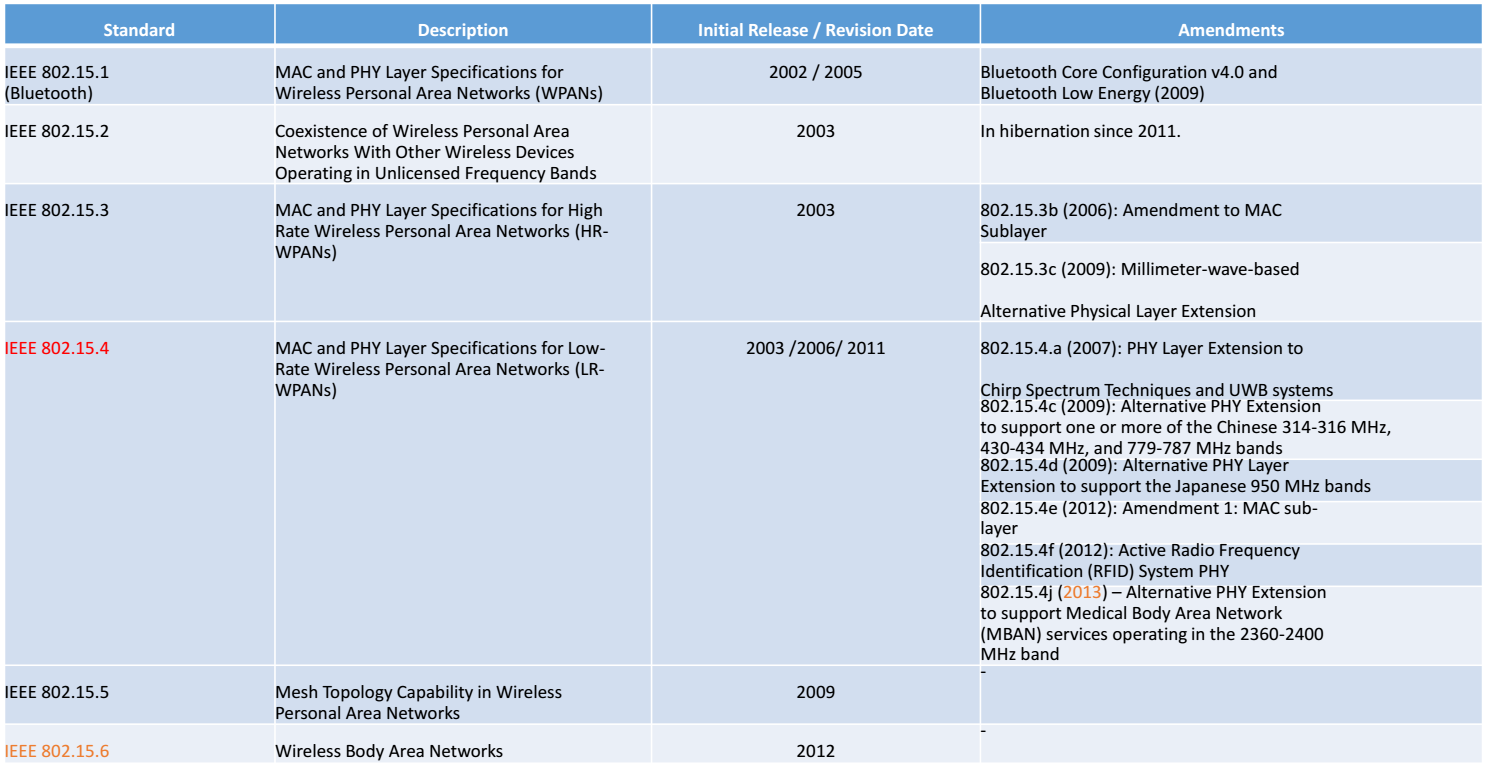
\includegraphics[width=1.05\textwidth,keepaspectratio]{figures/33.WirelessN/nancy2014}
	\caption{Members of the 802.15 family. Adapted from \cite{nancy2014} lecture presentation slides.}
	\label{fig:nancy2014}
\end{figure}

Based on figure \ref{fig:nancy2014}, the 802.15.4 is the standard that defines the \ac{PHY} and \ac{MAC} layers for low rate wireless personal area networks. It supports \textbf{full-function devices} (device capable of being the network coordinator or simple node and can have implemented complex network functionalities) and \textbf{reduced-function device} (limited devices with low-bandwidth limitations and limited or no-network intelligence). The possible network topologies are the following:

\begin{description}
	\item[Star ---] Each device in the network communicates with the full-function device network coordinator;
	
	\item[Peer-to-peer ---] All devices communicate with each other (if they are in the communication range). Sufficiently flexible to implement more complex topologies such as multi-hoping, cluster trees and mesh topologies;
	
	\item[Multi-hopping ---] This is a technique that allows the usage of two or more wireless nodes to convey data from a source to a destination;
	
	\item[Cluster trees] Topology to reduce the routing complexity where each node knows its parent node and all its child nodes. It has always only one single path between two nodes.
	
	\item[Wireless mesh] This technique allows data to be propagated along a path by hopping from node to node until it reaches its destination.
	
\end{description}

\subsubsection{802.15.4-based wireless standards}

Radmand et al. (2010) presents a comparison of wireless sensor standards for industrial applications, \cite{Radmand2010}. In figure \ref{fig:radmand2010} is present the overall schema of the wireless standards.


\begin{figure}[h!]
	\centering
	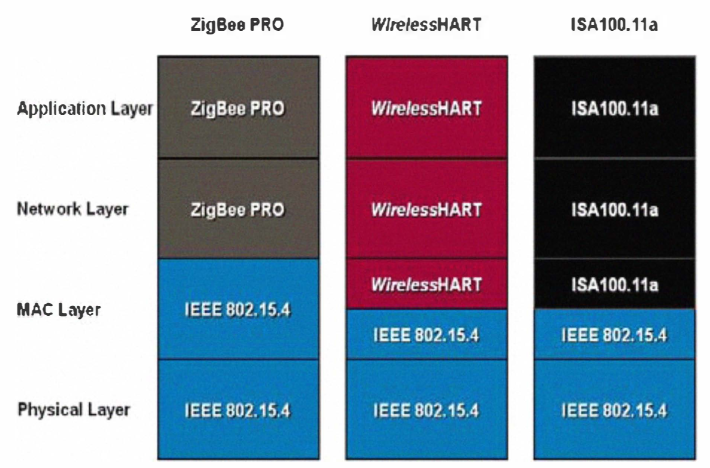
\includegraphics[width=0.6\textwidth,keepaspectratio]{figures/33.WirelessN/radmand2010}
	\caption{Overall schema of wireless standards. Adapted from \cite{Radmand2010}.}
	\label{fig:radmand2010}
\end{figure}


\subsection{Communication \ac{KPI}}
%\lipsum[4]
\label{subs:334}
According to Radmand et al. (2010), it is identified the following "Industrial Requirements" for the WSN's, \cite{Radmand2010}:

\begin{description}
	\item[Reliability ---] Reliability is a measurement of the transmission accuracy, in percentage, that evaluates the amount of data that reach its destination. This measurement uses the properties of data communication, acknowledge-based usually.
	
	\item[Latency ---] Latency is the measurement of the time delay and is defined as the time that a data packet takes to be transmitted from the source to the destination. The latency is directly related to the link quality and a high latency link is result of a link with high signal-to-noise ratio. 
	
	\item[Sensor Data Update Rates ---] This \ac{KPI} is not directly related with the communication link. However, the update rate of the sensor data affects the power consumption due to the increase of the processing effort. In a SYNC-based update rate, this \ac{KPI} is related to the frequency of the SYNC event.
	
	\item[Wireless Transmission Range ---] This \ac{KPI} is the maximum distance that a communication link supports the data transfer with a given reliability and in specific conditions (indoor/outdoor; line-of-sight (LOS)).
	
	\item[Power consumption ---] The power consumption is a measurement of the combination of the computational effort of the nodes and the transmission effort. It is directly related with the update rate as well as with the link quality and, if it exists, the routing activity in each node.
	
\end{description}

%\subsection{Emerging Technologies and Research Trends}

%%ver livro khan

\subsection{Network Simulators and Network Emulators}
\label{subs:335}

In this subsection is covered the network simulators. The usage of network simulators allows the modeling of various scenarios of real environment. However, pure network simulators avoid the interaction with real environment, which leads space for network emulators, as a hybrid method to combine simulation capabilities with hardware and software components of real networks. Therefore, in this subsection is referred the simulators that allows integration with hardware and software network components, to have an overview on the network emulators.

In figure \ref{fig:simul_VS_emul} is presented the framework on the mechanisms to evaluate the performance of networks.

\begin{figure}[h!]
	\centering
	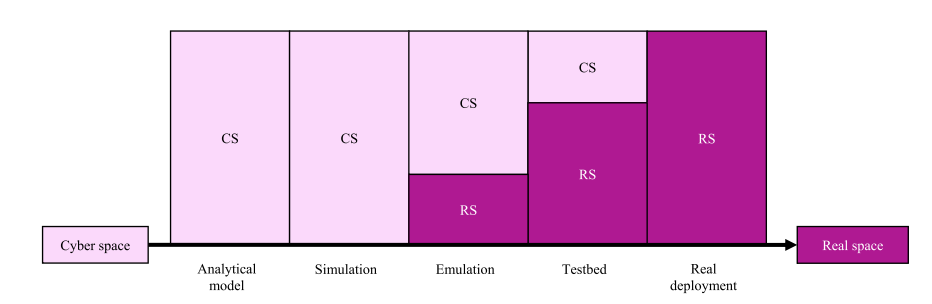
\includegraphics[width=1\textwidth,keepaspectratio]{figures/33.WirelessN/simul_VS_emul}
	\caption{Simulation \& emulation framework.}
	\label{fig:simul_VS_emul}
\end{figure}

An extensive review on simulation tools, made by \cite{nayyar2015}, is presented as following:

\begin{description}
	\setlength\itemsep{0.5em}
	%%1
	\item [NS-2 (network simulator-2)] 
	Object orientated discrete event simulator tool, based on two languages (C++ and OTcl). 
	
	%%2
	\item [NS-3 (network simulator-3)] 
	Written in pure C++, this simulator has been extensively explored in the literature with various modules like 802.15.4, 6LoWPAN and RPL available. With the usage of ns-3 in emulation mode, the implementation of real testbeds can be validated since it is possible to generate repeatable experimental results, with the usage of real-world network environment that includes all of the ns-3 tracing, logging, visualization and statistics gathering tools.
	
	%%3
	\item [OMNET++] 
	This simulator is based in C++ in the basic modules and uses Network DEscription (.NED) scripts to connect and assemble the simulation basic modules.

	%%4
	\item [J-Sim] 
	JavaSim Simulator has been developed in Java and it has several advantages to carry out large scale WSN simulations.

	%%5
	\item [Mannasim] 
	Is based on NS-2 to perform WSN simulations.

	%%6
	\item [SensorSim] 
	Similarly to Mannasim, this is a framework for WSN based on NS-2 simulator. However, currently it is not available to the public. 

	%%7
	\item [NRL Sensorsim] 
	This extension to NS-2 simulator is focused on WSN, similarly to SensorSim and Mannasim frameworks. Currently, it is no longer in development and does not have support.

	%%8
	\item [NCTUns 6.0] 
	On the field of network emulators, this software has the main advantage of using the real world Linux TCP/IP stack and implements almost every IEEE network standards. Last release was on 2010.

	%%9
	\item [SSFNet] 
	Java simulator designed especially for WSN's. Last release in 2004.

	%%10
	\item [GloMoSim] 
	Non-commercial simulator (the commercial version is \textit{"QualNet"}) designed for wireless and wired network systems.

	%%11
	\item [QualNet 7.0 + EXata 5] 
	Considered one of the most advanced simulator platform these days, QualNet enables a high fidelity virtual model of network, with an advanced GUI. It has a free academic version.

	%%12
	\item [sQualNet Simulator] 
	Is an extension of QualNet for sensor network specific models. 

	%%13
	\item [OPNET Modeler Suite] 
	Is a powerful collection with an interactive GUI to build network scenarios. It has a free academic edition. 

	%%14
	\item [SENSE] 
	Is a powerful sensor network simulator and emulator.

	%%15
	\item [DRMSim] 
	Is a Java-based software that enables large-scale network simulation.

	%%16
	\item [NetSim] 
	Is a simulator designed for protocol modeling, network research and development and defense applications.

	%%17
	\item [UWSim] 
	This simulator is designed for marine robotics research.

	%%18
	\item [Visual Sense] 
	This modeling and simulation software is designed for wireless and WSN applications, as an extension of Ptolemy II.

	%%19
	\item [Viptos] 
	Is an interface/bridge between TinyOS and Ptolemy II.

	%%20
	\item [PTOLEMY II] 
	Is an open source simulation software, based on Java and with actor-oriented design (where actors are software components, have a concurrent execution and communicate via interconnected ports)
	
	%%21
	\item [SENS] 
	This specific framework for WSN's simulator and emulator that uses a simplified sensor model.
	
	%%22
	\item [SHAWN]	
	Is a customizable sensor network simulator focused on the simulation of the effect caused by a phenomenon (not the phenomenon itself) with scalability and support for extremely large networks. According to SHAWN development repository, last contribution was on 2013.
		
	%%23
	\item [SIDnet-SWANS]
	This Java-based simulator was made to provide a simulation and proof-of-concept platform for application of WSN's.
	Latest version was released in 2011.
	
	%%24
	\item [WSim/Worldsens Simulator/WSNet Simulator]
	This simulator states for being an event-driven simulator for large scale wireless networks. Latest version was released in 2009.

	%%25
	\item [WSN Localization Simulator]
	This is a WSN location simulator stating for being easy, scalable and extendable to many/different localization schemes. It was released in 2013.
	
	%%26
	\item [NetTopo Simulator]
	This framework is an open source simulator designed in Java. Its main objective is to analyze various algorithms in WSN's. 
	
	%%27
	\item [SIDH]
	Is a Java-based simulator focused on the simulation of thousands of sensor nodes.
	
	%%28
	\item [PROWLER]
	The Probabilistic Wireless Sensor Network Simulator is a framework that runs under Matlab and is focused to TinyOS applications.
	
	%%29
	\item [Matlab/Simulink]
	With extensive usage by the research community, Matlab and Simulink software provides resourceful toolboxes for simulation of communication networks, being possible to build a complete WSN model system.
	
	%%30
	\item [PiccSIM]
	This simulation platform uses Matlab/Simuling and NS-2 for networked control systems (in particular wireless)
	
	%%31
	\item [LabVIEW]
	Various toolboxes to simulate WSN's are available with LabVIEW.
	
\end{description}


\subsubsection{Evaluation of network tools}

In the previous list, several tools for the evaluation of network performance was presented. Special attention is given for the tools that has large support either for implementation of several network technologies (wired and wireless) and, with this requirement, the following network simulators will be considered for further research:
	
\begin{itemize}
	\setlength\itemsep{-0.5em}
	\item NS-3;
	\item OMNET++;
	\item QualNet 7.0 + EXata 5;
	\item MatLab Simulink;
\end{itemize}



